\documentclass[lualatex,handout]{beamer}
\setbeamertemplate{footline}[frame number]
\usepackage{luatexja}
\usepackage{amsmath,amssymb}

%\usetheme{Berlin}
\usecolortheme{rose}

\usepackage{tikz}
\usepackage{pgfplots}
\pgfplotsset{compat=1.18}

%\usepackage[haranoaji]{luatexja-preset}
\usepackage[deluxe,ipaex]{luatexja-preset}
\renewcommand{\kanjifamilydefault}{\gtdefault}
%\setmainjfont{HaranoAjiGothic-Regular}

\usepackage{unicode-math}
%\setmathfont{Fira Math}
\setmathfont{STIX Two Math}
\setmathfont{STIX Two Math}[range=bfup/{Latin,latin,num,Greek,greek}]
\setmathfont{STIX Two Math}[range=bfit/{Latin,latin}]
\setmathfont{STIX Two Math}[range={"0000-"FFFF}]
\setmathrm{STIX Two Math}[StylisticSet=8]

%\usefonttheme{professionalfonts}

\usepackage{luacolor}

\newcommand{\mycolor}[2]{%
  \begingroup
  \colorlet{currentcolor}{.}%
  \color{#1}#2%
  \color{currentcolor}%
  \endgroup
}
\newcommand{\emm}[1]{\mycolor{red}{#1}}
\newcommand{\expt}[1]{\mathbb{E}\left[#1\right]}
\newcommand{\var}[1]{\mathbb{V}\left[#1\right]}
\newcommand{\cov}[1]{\mathsf{Cov}\left[#1\right]}
\newcommand{\vc}[1]{\mathsf{Var}\left[#1\right]}


\usepackage{xspace}
%\usepackage{bm}
%\newcommand\bm[1]{{\mathbf{#1}}}
\newcommand\dx{{\,\mathrm{d}x}}

\theoremstyle{definition}

\title{確率・統計基礎: 中心極限定理、正規分布}
\author{森 立平}
\date{}



\begin{document}
\begin{frame}[plain]
\maketitle
\end{frame}

\begin{frame}{大数の法則と集中不等式}

%確率変数$X_1,X_2,\dotsc,X_N$が\emm{独立}で\emm{同一の分布}に従うとき、
%独立同分布(independently and identically distributed (i.i.d.))であるという。

%\vspace{2em}
{このスライドでは$X_1,\dotsc,X_N$は i.i.d.で確率変数$X$と同分布であると仮定}する。

\vspace{2em}
集中不等式は
\begin{align*}
\Pr\left(\left|\left(\sum_{k=1}^NX_k\right) - N\expt{X}\right| \ge \emm{N}\epsilon\right)
\end{align*}
が指数関数的に小さいことを示している。

\vspace{2em}
今日は期待値の近くに注目し、
\begin{align*}
\Pr\left(\left|\left(\sum_{k=1}^NX_k\right) - N\expt{X}\right| \ge \emm{\sqrt{N}}\epsilon\right)
\end{align*}
について考えてみる
\end{frame}

\begin{frame}{二項分布}
\begin{align*}
\Pr(X = k) &= \binom{n}{k} p^k(1-p)^{n-k},\quad \emm{n=30},\, p=0.3.
\end{align*}
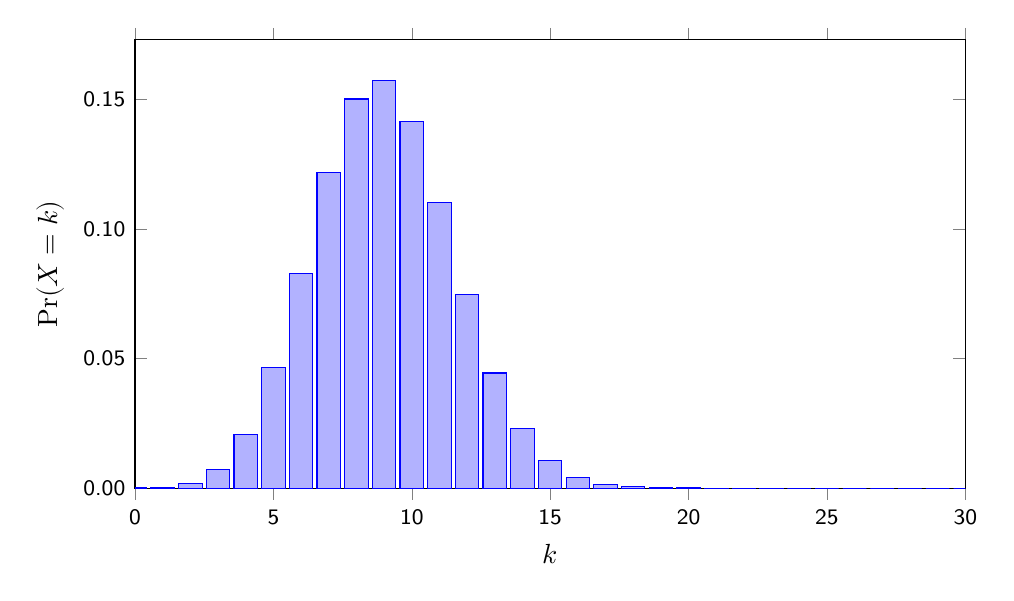
\begin{tikzpicture}[%
declare function={binom(\k,\n,\p)=\n!/(\k!*(\n-\k)!)*\p^\k*(1-\p)^(\n-\k);}]
\pgfmathsetmacro{\binomN}{30}
\begin{axis}[
    width=\textwidth, height=\axisdefaultheight,
    ylabel={$\Pr(X=k)$},
    xlabel={$k$},
    xmin=0, xmax=\binomN,
    ymin=0,
    scaled ticks = false,
    tick label style={/pgf/number format/assume math mode=true, font=\footnotesize\sffamily},
    yticklabel style={/pgf/number format/.cd, fixed, fixed zerofill, precision=2},
        domain=0:\binomN,samples at={0,1,...,\binomN},
    mark options={scale=0.75, blue},
    ybar, bar width = 8.5pt
        ]
%\addplot[ycomb] {binom(x,\binomN,0.3)};
\addplot {binom(x,\binomN,0.3)};
\end{axis}
\end{tikzpicture}
\end{frame}

\begin{frame}{二項分布}
\begin{align*}
\Pr(X = k) &= \binom{n}{k} p^k(1-p)^{n-k},\quad \emm{n=60},\, p=0.3.
\end{align*}
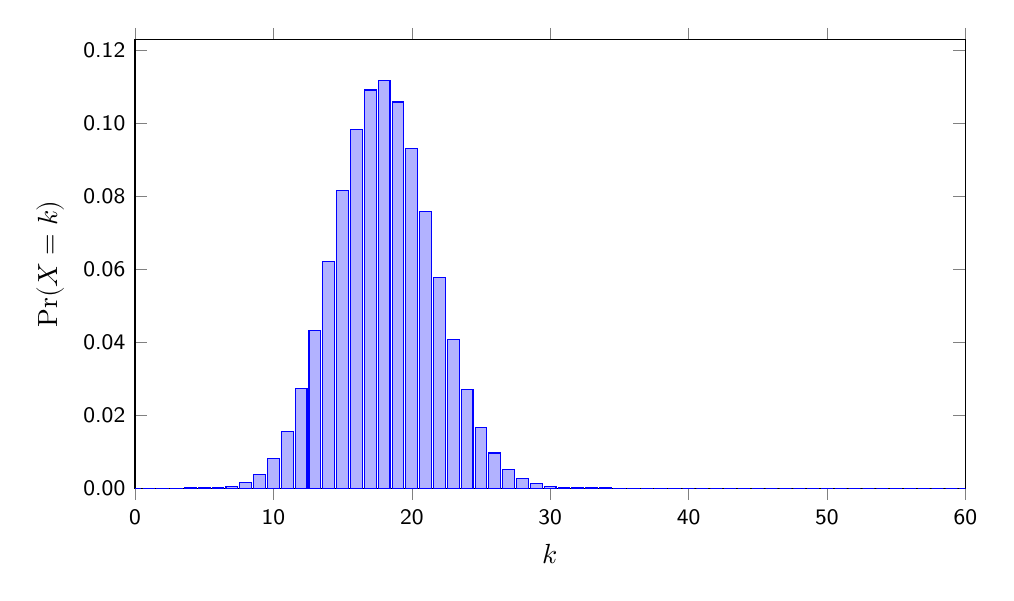
\begin{tikzpicture}[%
declare function={binom(\k,\n,\p)=\n!/(\k!*(\n-\k)!)*\p^\k*(1-\p)^(\n-\k);}]
\pgfmathsetmacro{\binomN}{60}
\begin{axis}[
    width=\textwidth, height=\axisdefaultheight,
    ylabel={$\Pr(X=k)$},
    xlabel={$k$},
    xmin=0, xmax=\binomN,
    ymin=0,
    scaled ticks = false,
    tick label style={/pgf/number format/assume math mode=true, font=\footnotesize\sffamily},
    yticklabel style={/pgf/number format/.cd, fixed, fixed zerofill, precision=2},
        domain=0:\binomN,samples at={0,1,...,\binomN},
    mark options={scale=0.75, blue},
    ybar, bar width = 4.25pt
        ]
%\addplot[ycomb] {binom(x,\binomN,0.3)};
\addplot {binom(x,\binomN,0.3)};
\end{axis}
\end{tikzpicture}
\end{frame}

\begin{frame}{二項分布}
\begin{align*}
\Pr(X = k) &= \binom{n}{k} p^k(1-p)^{n-k},\quad \emm{n=120},\, p=0.3.
\end{align*}
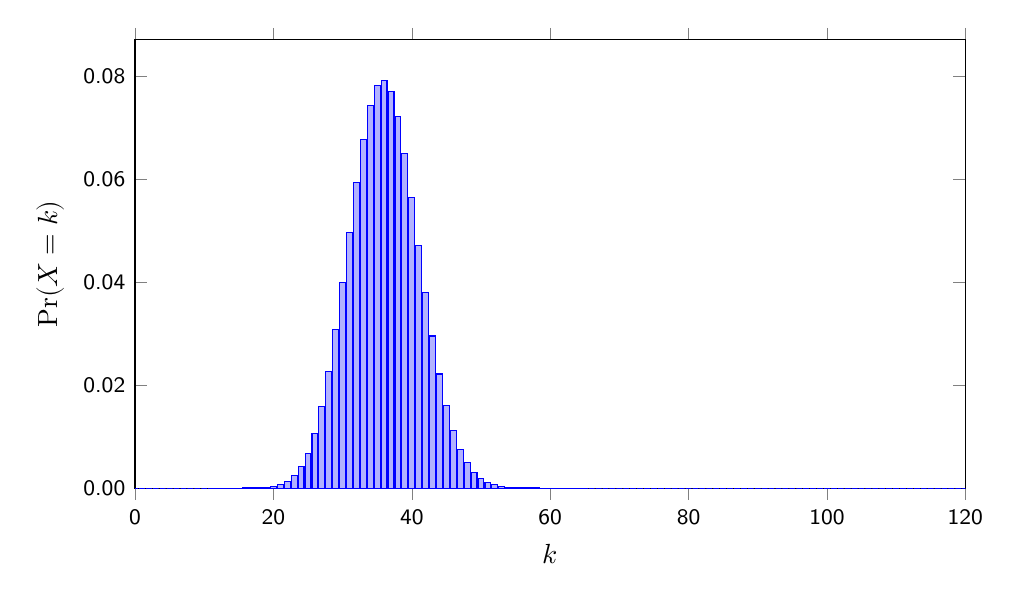
\begin{tikzpicture}[%
declare function={binom(\k,\n,\p)=\n!/(\k!*(\n-\k)!)*\p^\k*(1-\p)^(\n-\k);}]
\pgfmathsetmacro{\binomN}{120}
\begin{axis}[
    width=\textwidth, height=\axisdefaultheight,
    ylabel={$\Pr(X=k)$},
    xlabel={$k$},
    xmin=0, xmax=\binomN,
    ymin=0,
    scaled ticks = false,
    tick label style={/pgf/number format/assume math mode=true, font=\footnotesize\sffamily},
    yticklabel style={/pgf/number format/.cd, fixed, fixed zerofill, precision=2},
        domain=0:\binomN,samples at={0,1,...,\binomN},
    mark options={scale=0.75, blue},
    ybar, bar width = 2.125pt
        ]
%\addplot[ycomb] {binom(x,\binomN,0.3)};
\addplot {binom(x,\binomN,0.3)};
\end{axis}
\end{tikzpicture}
\end{frame}

\begin{frame}{二項分布}
\begin{align*}
\Pr(X = k) &= \binom{n}{k} p^k(1-p)^{n-k},\quad \emm{n=240},\, p=0.3.
\end{align*}
\begin{tikzpicture}[%
declare function={binom(\k,\n,\p)=\n!/(\k!*(\n-\k)!)*\p^\k*(1-\p)^(\n-\k);}]
\pgfmathsetmacro{\binomN}{240}
\pgfmathsetmacro{\p}{0.3}
\begin{axis}[
    width=\textwidth, height=\axisdefaultheight,
    ylabel={$\Pr(X=k)$},
    xlabel={$k$},
    xmin=0, xmax=\binomN,
    ymin=0,
    scaled ticks = false,
    tick label style={/pgf/number format/assume math mode=true, font=\footnotesize\sffamily},
    yticklabel style={/pgf/number format/.cd, fixed, fixed zerofill, precision=2},
        domain=0:\binomN,samples at={0,1,...,\binomN},
    mark options={scale=0.75, blue},
    ybar, bar width = .75pt
        ]
%\addplot[ycomb] {binom(x,\binomN,0.3)};
%\addplot {binom(x,\binomN,0.3)};
\addplot[domain=0:\binomN, color=blue, samples={\binomN+1}, thick] gnuplot { exp(lgamma(\binomN+1) - lgamma(x+1) - lgamma(\binomN-x+1) + x*log(\p) + (\binomN-x)*log(1-\p)) with impulses};
\end{axis}
\end{tikzpicture}
\end{frame}

\begin{frame}{二項分布}
\begin{align*}
\Pr(X = k) &= \binom{n}{k} p^k(1-p)^{n-k},\quad \emm{n=480},\, p=0.3.
\end{align*}
\begin{tikzpicture}[%
declare function={binom(\k,\n,\p)=\n!/(\k!*(\n-\k)!)*\p^\k*(1-\p)^(\n-\k);}]
\pgfmathsetmacro{\binomN}{480}
\pgfmathsetmacro{\p}{0.3}
\begin{axis}[
    width=\textwidth, height=\axisdefaultheight,
    ylabel={$\Pr(X=k)$},
    xlabel={$k$},
    xmin=0, xmax=\binomN,
    ymin=0,
    scaled ticks = false,
    tick label style={/pgf/number format/assume math mode=true, font=\footnotesize\sffamily},
    yticklabel style={/pgf/number format/.cd, fixed, fixed zerofill, precision=2},
        domain=0:\binomN,samples at={0,1,...,\binomN},
    mark options={scale=0.75, blue},
    ybar, bar width = .375pt
        ]
%\addplot[ycomb] {binom(x,\binomN,0.3)};
%\addplot {binom(x,\binomN,0.3)};
\addplot[domain=0:\binomN, color=blue, samples={\binomN+1}, thick] gnuplot { exp(lgamma(\binomN+1) - lgamma(x+1) - lgamma(\binomN-x+1) + x*log(\p) + (\binomN-x)*log(1-\p)) with impulses};
%\addplot[domain=0:\binomN, thick] gnuplot {x};
\end{axis}
\end{tikzpicture}
\end{frame}

\begin{frame}{二項分布}
\begin{align*}
\Pr(X = k) &= \binom{n}{k} p^k(1-p)^{n-k},\quad \emm{n=1000},\, p=0.3.
\end{align*}
\begin{tikzpicture}[%
declare function={binom(\k,\n,\p)=\n!/(\k!*(\n-\k)!)*\p^\k*(1-\p)^(\n-\k);}]
\pgfmathsetmacro{\binomN}{1000}
\pgfmathsetmacro{\p}{0.3}
\begin{axis}[
    width=\textwidth, height=\axisdefaultheight,
    ylabel={$\Pr(X=k)$},
    xlabel={$k$},
    xmin=0, xmax=\binomN,
    ymin=0,
    scaled ticks = false,
    tick label style={/pgf/number format/assume math mode=true, font=\footnotesize\sffamily},
    yticklabel style={/pgf/number format/.cd, fixed, fixed zerofill, precision=2},
        domain=0:\binomN,samples at={0,1,...,\binomN},
    mark options={scale=0.75, blue},
    ybar, bar width = .375pt
        ]
%\addplot[ycomb] {binom(x,\binomN,0.3)};
%\addplot {binom(x,\binomN,0.3)};
\addplot[domain=0:\binomN, color=blue, samples={\binomN+1}, thick] gnuplot { exp(lgamma(\binomN+1) - lgamma(x+1) - lgamma(\binomN-x+1) + x*log(\p) + (\binomN-x)*log(1-\p)) with impulses};
%\addplot[domain=0:\binomN, thick] gnuplot {x};
\end{axis}
\end{tikzpicture}
\end{frame}

\begin{frame}{二項分布}
\begin{align*}
\Pr(X = k) &= \binom{n}{k} p^k(1-p)^{n-k},\quad \emm{n=10000},\, p=0.3.
\end{align*}
\begin{tikzpicture}[%
declare function={binom(\k,\n,\p)=\n!/(\k!*(\n-\k)!)*\p^\k*(1-\p)^(\n-\k);}]
\pgfmathsetmacro{\binomN}{10000}
\pgfmathsetmacro{\p}{0.3}
\begin{axis}[
    width=\textwidth, height=\axisdefaultheight,
    ylabel={$\Pr(X=k)$},
    xlabel={$k$},
    xmin=0, xmax=\binomN,
    ymin=0,
    scaled ticks = false,
    tick label style={/pgf/number format/assume math mode=true, font=\footnotesize\sffamily},
    yticklabel style={/pgf/number format/.cd, fixed, fixed zerofill, precision=3},
        domain=0:\binomN,samples at={0,1,...,\binomN},
    mark options={scale=0.75, blue},
    ybar, bar width = .375pt
        ]
%\addplot[ycomb] {binom(x,\binomN,0.3)};
%\addplot {binom(x,\binomN,0.3)};
\addplot[domain=0:\binomN, color=blue, samples={\binomN+1}, thick] gnuplot { exp(lgamma(\binomN+1) - lgamma(x+1) - lgamma(\binomN-x+1) + x*log(\p) + (\binomN-x)*log(1-\p)) with impulses};
%\addplot[domain=0:\binomN, thick] gnuplot {x};
\end{axis}
\end{tikzpicture}
\end{frame}

\if0
\begin{frame}{二項分布}
\begin{align*}
\Pr(X = k) &= \binom{n}{k} p^k(1-p)^{n-k},\quad \emm{n=20000},\, p=0.3.
\end{align*}
\begin{tikzpicture}[%
declare function={binom(\k,\n,\p)=\n!/(\k!*(\n-\k)!)*\p^\k*(1-\p)^(\n-\k);}]
\pgfmathsetmacro{\binomN}{20000}
\pgfmathsetmacro{\p}{0.3}
\begin{axis}[
    width=\textwidth, height=\axisdefaultheight,
    ylabel={$\Pr(X=k)$},
    xlabel={$k$},
    xmin=0, xmax=\binomN,
    ymin=0,
    scaled ticks = false,
    tick label style={/pgf/number format/assume math mode=true, font=\footnotesize\sffamily},
    yticklabel style={/pgf/number format/.cd, fixed, fixed zerofill, precision=2},
        domain=0:\binomN,samples at={0,1,...,\binomN},
    mark options={scale=0.75, blue},
    ybar, bar width = .375pt
        ]
%\addplot[ycomb] {binom(x,\binomN,0.3)};
%\addplot {binom(x,\binomN,0.3)};
\addplot[domain=0:\binomN, color=blue, samples={\binomN+1}, thick] gnuplot { exp(lgamma(\binomN+1) - lgamma(x+1) - lgamma(\binomN-x+1) + x*log(\p) + (\binomN-x)*log(1-\p)) with impulses};
%\addplot[domain=0:\binomN, thick] gnuplot {x};
\end{axis}
\end{tikzpicture}
\end{frame}
\fi

\begin{frame}{二項分布}
\begin{align*}
\Pr(X = k) &= \binom{n}{k} p^k(1-p)^{n-k},\quad \emm{n=30},\, p=0.3.
\end{align*}
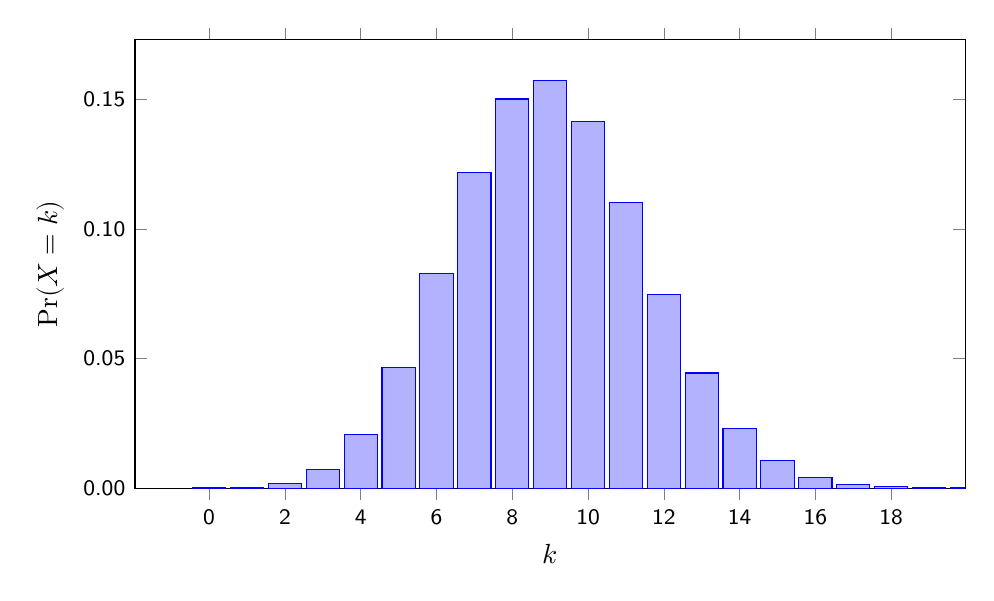
\begin{tikzpicture}[%
declare function={binom(\k,\n,\p)=\n!/(\k!*(\n-\k)!)*\p^\k*(1-\p)^(\n-\k);}]
\pgfmathsetmacro{\binomN}{30}
\pgfmathsetmacro{\p}{0.3}
\pgfmathsetmacro{\expect}{{\p*\binomN}}
\pgfmathsetmacro{\deviat}{{2*sqrt(\binomN)}}
\begin{axis}[
    width=\textwidth, height=\axisdefaultheight,
    ylabel={$\Pr(X=k)$},
    xlabel={$k$},
    xmin={\expect-\deviat}, xmax={\expect+\deviat},
    ymin=0,
    scaled ticks = false,
    tick label style={/pgf/number format/assume math mode=true, font=\footnotesize\sffamily},
    yticklabel style={/pgf/number format/.cd, fixed, fixed zerofill, precision=2},
        domain=0:\binomN,samples at={0,1,...,\binomN},
    mark options={scale=0.75, blue},
    ybar, bar width = 12pt
        ]
%\addplot[ycomb] {binom(x,\binomN,0.3)};
\addplot {binom(x,\binomN,\p)};
\end{axis}
\end{tikzpicture}
\end{frame}

\begin{frame}{二項分布}
\begin{align*}
\Pr(X = k) &= \binom{n}{k} p^k(1-p)^{n-k},\quad \emm{n=60},\, p=0.3.
\end{align*}
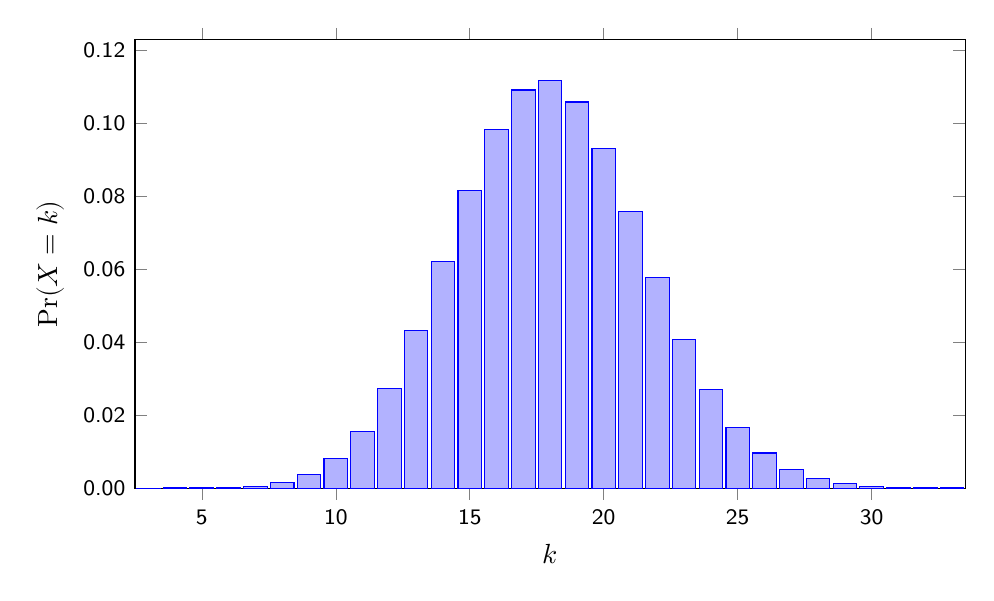
\begin{tikzpicture}[%
declare function={binom(\k,\n,\p)=\n!/(\k!*(\n-\k)!)*\p^\k*(1-\p)^(\n-\k);}]
\pgfmathsetmacro{\binomN}{60}
\pgfmathsetmacro{\p}{0.3}
\pgfmathsetmacro{\expect}{{\p*\binomN}}
\pgfmathsetmacro{\deviat}{{2*sqrt(\binomN)}}
\begin{axis}[
    width=\textwidth, height=\axisdefaultheight,
    ylabel={$\Pr(X=k)$},
    xlabel={$k$},
    xmin={\expect-\deviat}, xmax={\expect+\deviat},
    ymin=0,
    scaled ticks = false,
    tick label style={/pgf/number format/assume math mode=true, font=\footnotesize\sffamily},
    yticklabel style={/pgf/number format/.cd, fixed, fixed zerofill, precision=2},
        domain=0:\binomN,samples at={0,1,...,\binomN},
    mark options={scale=0.75, blue},
    ybar, bar width = 8.5pt
        ]
%\addplot[ycomb] {binom(x,\binomN,0.3)};
\addplot {binom(x,\binomN,\p)};
\end{axis}
\end{tikzpicture}
\end{frame}

\begin{frame}{二項分布}
\begin{align*}
\Pr(X = k) &= \binom{n}{k} p^k(1-p)^{n-k},\quad \emm{n=120},\, p=0.3.
\end{align*}
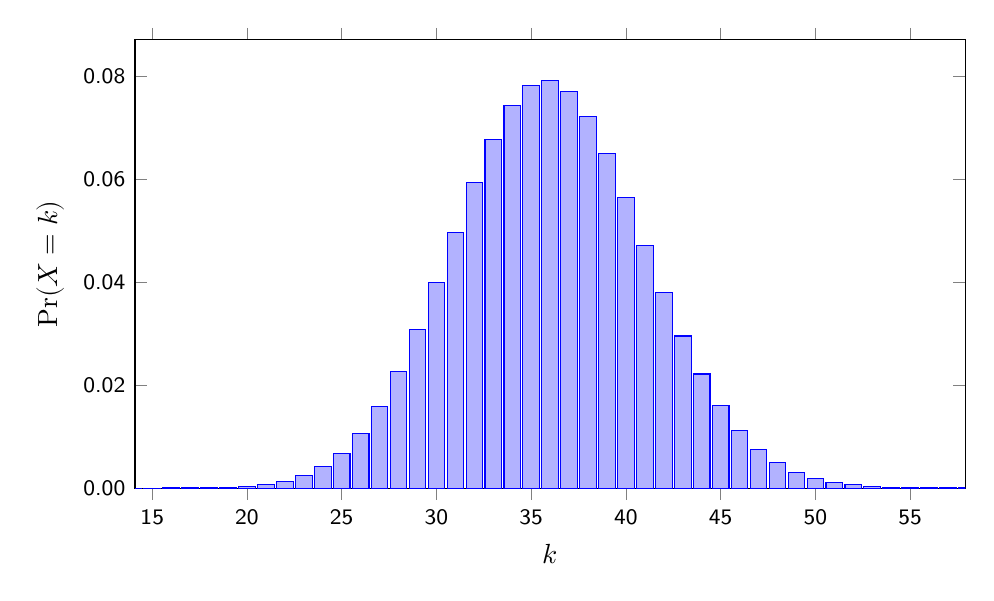
\begin{tikzpicture}[%
declare function={binom(\k,\n,\p)=\n!/(\k!*(\n-\k)!)*\p^\k*(1-\p)^(\n-\k);}]
\pgfmathsetmacro{\binomN}{120}
\pgfmathsetmacro{\p}{0.3}
\pgfmathsetmacro{\expect}{{\p*\binomN}}
\pgfmathsetmacro{\deviat}{{2*sqrt(\binomN)}}
\begin{axis}[
    width=\textwidth, height=\axisdefaultheight,
    ylabel={$\Pr(X=k)$},
    xlabel={$k$},
    xmin={\expect-\deviat}, xmax={\expect+\deviat},
    ymin=0,
    scaled ticks = false,
    tick label style={/pgf/number format/assume math mode=true, font=\footnotesize\sffamily},
    yticklabel style={/pgf/number format/.cd, fixed, fixed zerofill, precision=2},
        domain=0:\binomN,samples at={0,1,...,\binomN},
    mark options={scale=0.75, blue},
    ybar, bar width = 6pt
        ]
%\addplot[ycomb] {binom(x,\binomN,0.3)};
\addplot {binom(x,\binomN,\p)};
\end{axis}
\end{tikzpicture}
\end{frame}

\begin{frame}{二項分布}
\begin{align*}
\Pr(X = k) &= \binom{n}{k} p^k(1-p)^{n-k},\quad \emm{n=240},\, p=0.3.
\end{align*}
\begin{tikzpicture}[%
declare function={binom(\k,\n,\p)=\n!/(\k!*(\n-\k)!)*\p^\k*(1-\p)^(\n-\k);}]
\pgfmathsetmacro{\binomN}{240}
\pgfmathsetmacro{\p}{0.3}
\pgfmathsetmacro{\expect}{{\p*\binomN}}
\pgfmathsetmacro{\deviat}{{2*sqrt(\binomN)}}
\begin{axis}[
    width=\textwidth, height=\axisdefaultheight,
    ylabel={$\Pr(X=k)$},
    xlabel={$k$},
    xmin={\expect-\deviat}, xmax={\expect+\deviat},
    ymin=0,
    scaled ticks = false,
    tick label style={/pgf/number format/assume math mode=true, font=\footnotesize\sffamily},
    yticklabel style={/pgf/number format/.cd, fixed, fixed zerofill, precision=2},
        domain=0:\binomN,samples at={0,1,...,\binomN},
    mark options={scale=0.75, blue},
    ybar, bar width = 4.25pt
        ]
%\addplot[ycomb] {binom(x,\binomN,0.3)};
%\addplot {binom(x,\binomN,\p)};
\addplot[domain=0:\binomN, color=blue, samples={\binomN+1}, thick] gnuplot { exp(lgamma(\binomN+1) - lgamma(x+1) - lgamma(\binomN-x+1) + x*log(\p) + (\binomN-x)*log(1-\p)) with impulses};
\end{axis}
\end{tikzpicture}
\end{frame}

\begin{frame}{二項分布}
\begin{align*}
\Pr(X = k) &= \binom{n}{k} p^k(1-p)^{n-k},\quad \emm{n=480},\, p=0.3.
\end{align*}
\begin{tikzpicture}[%
declare function={binom(\k,\n,\p)=\n!/(\k!*(\n-\k)!)*\p^\k*(1-\p)^(\n-\k);}]
\pgfmathsetmacro{\binomN}{480}
\pgfmathsetmacro{\p}{0.3}
\pgfmathsetmacro{\expect}{{\p*\binomN}}
\pgfmathsetmacro{\deviat}{{2*sqrt(\binomN)}}
\begin{axis}[
    width=\textwidth, height=\axisdefaultheight,
    ylabel={$\Pr(X=k)$},
    xlabel={$k$},
    xmin={\expect-\deviat}, xmax={\expect+\deviat},
    ymin=0,
    scaled ticks = false,
    tick label style={/pgf/number format/assume math mode=true, font=\footnotesize\sffamily},
    yticklabel style={/pgf/number format/.cd, fixed, fixed zerofill, precision=2},
        domain=0:\binomN,samples at={0,1,...,\binomN},
    mark options={scale=0.75, blue},
    ybar, bar width = 3pt
        ]
%\addplot[ycomb] {binom(x,\binomN,0.3)};
%\addplot {binom(x,\binomN,\p)};
%\addplot[domain={\expect-\deviat}:{\expect+\deviat}, color=blue, samples={2*\deviat+1}, thick] gnuplot { exp(lgamma(\binomN+1) - lgamma(x+1) - lgamma(\binomN-x+1) + x*log(\p) + (\binomN-x)*log(1-\p)) with impulses};
\addplot[domain=0:\binomN, color=blue, samples={\binomN+1}, thick] gnuplot { exp(lgamma(\binomN+1) - lgamma(x+1) - lgamma(\binomN-x+1) + x*log(\p) + (\binomN-x)*log(1-\p)) with impulses};
\end{axis}
\end{tikzpicture}
\end{frame}

\begin{frame}{二項分布}
\begin{align*}
\Pr(X = k) &= \binom{n}{k} p^k(1-p)^{n-k},\quad \emm{n=1000},\, p=0.3.
\end{align*}
\begin{tikzpicture}[%
declare function={binom(\k,\n,\p)=\n!/(\k!*(\n-\k)!)*\p^\k*(1-\p)^(\n-\k);}]
\pgfmathsetmacro{\binomN}{1000}
\pgfmathsetmacro{\p}{0.3}
\pgfmathsetmacro{\expect}{{\p*\binomN}}
\pgfmathsetmacro{\deviat}{{2*sqrt(\binomN)}}
\begin{axis}[
    width=\textwidth, height=\axisdefaultheight,
    ylabel={$\Pr(X=k)$},
    xlabel={$k$},
    xmin={\expect-\deviat}, xmax={\expect+\deviat},
    ymin=0,
    scaled ticks = false,
    tick label style={/pgf/number format/assume math mode=true, font=\footnotesize\sffamily},
    yticklabel style={/pgf/number format/.cd, fixed, fixed zerofill, precision=2},
        domain=0:\binomN,samples at={0,1,...,\binomN},
    mark options={scale=0.75, blue},
    ybar, bar width = 2pt
        ]
%\addplot[ycomb] {binom(x,\binomN,0.3)};
%\addplot {binom(x,\binomN,\p)};
%\addplot[domain={\expect-\deviat}:{\expect+\deviat}, color=blue, samples={2*\deviat+1}, thick] gnuplot { exp(lgamma(\binomN+1) - lgamma(x+1) - lgamma(\binomN-x+1) + x*log(\p) + (\binomN-x)*log(1-\p)) with impulses};
\addplot[domain=0:\binomN, color=blue, samples={\binomN+1}, thick] gnuplot { exp(lgamma(\binomN+1) - lgamma(x+1) - lgamma(\binomN-x+1) + x*log(\p) + (\binomN-x)*log(1-\p)) with impulses};
\end{axis}
\end{tikzpicture}
\end{frame}

\begin{frame}{二項分布}
\begin{align*}
\Pr(X = k) &= \binom{n}{k} p^k(1-p)^{n-k},\quad \emm{n=10000},\, p=0.3.
\end{align*}
\begin{tikzpicture}[%
declare function={binom(\k,\n,\p)=\n!/(\k!*(\n-\k)!)*\p^\k*(1-\p)^(\n-\k);}]
\pgfmathsetmacro{\binomN}{10000}
\pgfmathsetmacro{\p}{0.3}
\pgfmathsetmacro{\expect}{{\p*\binomN}}
\pgfmathsetmacro{\deviat}{{2*sqrt(\binomN)}}
\begin{axis}[
    width=\textwidth, height=\axisdefaultheight,
    ylabel={$\Pr(X=k)$},
    xlabel={$k$},
    xmin={\expect-\deviat}, xmax={\expect+\deviat},
    ymin=0,
    scaled ticks = false,
    tick label style={/pgf/number format/assume math mode=true, font=\footnotesize\sffamily},
    yticklabel style={/pgf/number format/.cd, fixed, fixed zerofill, precision=3},
        domain=0:\binomN,samples at={0,1,...,\binomN},
    mark options={scale=0.75, blue},
    ybar, bar width = .4pt
        ]
%\addplot[ycomb] {binom(x,\binomN,0.3)};
%\addplot {binom(x,\binomN,\p)};
%\addplot[domain={\expect-\deviat}:{\expect+\deviat}, color=blue, samples={2*\deviat+1}, thick] gnuplot { exp(lgamma(\binomN+1) - lgamma(x+1) - lgamma(\binomN-x+1) + x*log(\p) + (\binomN-x)*log(1-\p)) with impulses};
\addplot[domain=0:\binomN, color=blue, samples={\binomN+1}, thick] gnuplot { exp(lgamma(\binomN+1) - lgamma(x+1) - lgamma(\binomN-x+1) + x*log(\p) + (\binomN-x)*log(1-\p)) with impulses};
\end{axis}
\end{tikzpicture}
\end{frame}

\if0
\begin{frame}{二項分布}
\begin{align*}
\Pr(X = k) &= \binom{n}{k} p^k(1-p)^{n-k},\quad \emm{n=10000},\, p=0.3.
\end{align*}
\begin{tikzpicture}[%
declare function={binom(\k,\n,\p)=\n!/(\k!*(\n-\k)!)*\p^\k*(1-\p)^(\n-\k);}]
\pgfmathsetmacro{\binomN}{10000}
\pgfmathsetmacro{\p}{0.3}
\pgfmathsetmacro{\expect}{{\p*\binomN}}
\pgfmathsetmacro{\deviat}{{sqrt(\binomN)}}
\begin{axis}[
    width=\textwidth, height=\axisdefaultheight,
    ylabel={$\Pr(X=k)$},
    xlabel={$k$},
    xmin={\expect-\deviat}, xmax={\expect+\deviat},
    ymin=0,
    scaled ticks = false,
    tick label style={/pgf/number format/assume math mode=true, font=\footnotesize\sffamily},
    yticklabel style={/pgf/number format/.cd, fixed, fixed zerofill, precision=3},
        domain=0:\binomN,samples at={0,1,...,\binomN},
    mark options={scale=0.75, blue},
    ybar, bar width = .4pt
        ]
%\addplot[ycomb] {binom(x,\binomN,0.3)};
%\addplot {binom(x,\binomN,\p)};
%\addplot[domain={\expect-\deviat}:{\expect+\deviat}, color=blue, samples={2*\deviat+1}, thick] gnuplot { exp(lgamma(\binomN+1) - lgamma(x+1) - lgamma(\binomN-x+1) + x*log(\p) + (\binomN-x)*log(1-\p)) with impulses};
\addplot[domain=0:\binomN, color=blue, samples={\binomN+1}, thick] gnuplot { exp(lgamma(\binomN+1) - lgamma(x+1) - lgamma(\binomN-x+1) + x*log(\p) + (\binomN-x)*log(1-\p)) with impulses};
%\addplot {exp(-(x-\expect)^2/(2*sqrt(\binomN)))};
\end{axis}
\end{tikzpicture}
\end{frame}
\fi

\begin{frame}{中心極限定理}
\small
\begin{theorem}[中心極限定理]
$X$が分散を持つと仮定する。
\begin{align*}
\lim_{N\to\infty}\Pr\left(\frac{\left(\sum_{k=1}^N X_k\right)-N\expt{X}}{\sqrt{\var{X}N}} \le x\right) &= \Phi(x)
=\frac1{\sqrt{2\pi}}\int_{-\infty}^x\mathrm{e}^{-\frac{t^2}2}\mathrm{d}t
\end{align*}
\end{theorem}
\begin{align*}
Y_k&:= \frac{X_k-\expt{X}}{\sqrt{\var{X}}}\qquad \text{for } k=1,2,\dotsc,N
\end{align*}
は$X_k$を期待値0、分散1に正規化した確率変数である。
中心極限定理の主張は
\begin{align*}
\lim_{N\to\infty}\Pr\left(\frac{\sum_{k=1}^N Y_k}{\sqrt{N}} \le x\right) &= \Phi(x)
\end{align*}
である。$N$で割るのではなくて$\sqrt{N}$で割ることで大数の法則よりも細かい部分を見ている。
\end{frame}

\begin{frame}{特性関数}
\begin{definition}[特性関数]
確率変数$X$の\emm{特性関数}$\varphi_X\colon\mathbb{R}\to\mathbb{C}$を以下で定義する。
\begin{align*}
\varphi_X(t) &:= \expt{\mathrm{e}^{\emm{i}tX}}.
\end{align*}
\end{definition}
モーメント母関数は存在するとは限らないが特性関数は(定義域を$\mathbb{R}$として)\emm{常に存在}する。

\vspace{2em}
$X$と$Y$の分布が同じ$\emm{\iff}\varphi_X=\varphi_Y$ (ルベーグ積分に基づいた議論が必要).

\vspace{2em}
$X$が$k$次モーメントを持つ$\iff$$\varphi_X$は0で$k$回微分できる。
\begin{align*}
\left.\frac{\mathrm{d}^k\varphi_X(t)}{\mathrm{d}t^k}\right|_{t=0} &= i^k \expt{X^k}.
\end{align*}

%\vspace{1em}
%第二特性関数
%\begin{align*}
%H_X(t) &:= \log\expt{\mathrm{e}^{itX}}
%\end{align*}
\end{frame}

\begin{frame}{$X$と$Y$の分布が同じ$\iff\varphi_X=\varphi_Y$ (像が有限の場合)}
確率変数$X$の像$\mathrm{Image}(X)$が\emm{有限集合}のとき、
\begin{align*}
\varphi_X(t) &= \sum_{k\in \mathrm{Image}(X)} \Pr(X = k) \mathrm{e}^{itk}
\end{align*}
ここで、$\mathrm{Image}(X)$の最小値と最大値をそれぞれ$k_\mathsf{min}$と$k_\mathsf{max}$とおくと、
$k_\mathsf{max}-k_\mathsf{min}$次多項式$Q_X$を以下のように定義する。
\begin{align*}
Q_X(x) &= \sum_{k\in \mathrm{Image}(X)} \Pr(X = k) x^{k-k_{\mathsf{min}}}
\end{align*}
このとき、$Q_X(\mathrm{e}^{it}) = \varphi_X(t) \mathrm{e}^{-itk_\mathsf{min}}$である。
一般的に\emm{$n$次多項式は異なる$(n+1)$点での値から一意に定まる}(Vandermonde行列の正則性)。
よって特性関数から多項式$Q_X$が一意に定まり、$\Pr(X=k)$が一意に定まる。

\begin{center}
確率質量関数から特性関数への写像が\emm{単射}であることが分かった。
これは一般の確率変数について(確率密度関数が存在しない場合でも)成り立つ。
%(レヴィの連続性定理)
\end{center}
%\begin{align*}
%&\sum_{t} \varphi_X(t) \mathrm{e}^{-itu}\\
%=&\sum_{t} \sum_{k\in \mathrm{Im}(X)} \Pr(X = k) \mathrm{e}^{itk} \mathrm{e}^{-itu}\\
%=& \sum_{k\in \mathrm{Im}(X)} \Pr(X = k)\left(\sum_{t} \mathrm{e}^{it(k-u)}\right)
%\end{align*}
\end{frame}

\begin{frame}{おまけ: Vandermonde行列の正則性}
\footnotesize
\begin{definition}[Vandermonde行列]
$x_0,\x_1,\dotsc,x_N\in\mathbb{C}$について、Vandermonde行列は以下で定義される。
\begin{align*}
V(x_0,x_1,\dotsc,x_N)&:=
\begin{bmatrix}
1&x_0&x_0^2&\cdots&x_0^N\\
1&x_1&x_1^2&\cdots&x_1^N\\
\vdots\\
1&x_N&x_N^2&\cdots&x_N^N\\
\end{bmatrix}.
\end{align*}
\end{definition}
Vandermonde行列は多項式の係数から評価点への写像を表す。
\begin{lemma}
$x_0,x_1,\dotsc,x_N\in\mathbb{C}$が互いに異なるとき、$V(x_0,\dotsc,x_N)$は正則である。
\end{lemma}
\begin{proof}
$x_0,x_1,\dotsc,x_N\in\mathbb{C}$が互いに異なるとき、$\ker(V(x_0,\dotsc,x_N))=\{0\}$を示せばよい。
ある$b\in\mathbb{C}^{N+1}$について$V(x_0,\dotsc,x_N) b = 0$のとき、高々$N$次の多項式を$B(x):=\sum_{k=0}^N b_k x^k$と定義する。この多項式は少なくとも$N+1$個の根$x_0,\dotsc,x_N$を持つ。高々$N$次の非ゼロ多項式は相異なる根を高々$N$個持つため、$B$は零多項式であり、$b=0$である。
\end{proof}
\end{frame}

\if0
\begin{frame}{標準コーシー分布の特性関数}
\begin{align*}
p(x) &= \frac1{\pi(1+x^2)}
\end{align*}
\begin{align*}
\expt{\mathrm{e}^{itX}} &= \int_{-\infty}^\infty \mathrm{e}^{itx}\frac1{\pi(1+x^2)}\mathrm{d}x\\
&= \int_{-\infty}^\infty \mathrm{e}^{itx}\frac1{\pi(x-i)(x+i)}\mathrm{d}x\\
\end{align*}
\end{frame}
\fi

\begin{frame}{分布の収束と特性関数の収束}
\begin{theorem}[レヴィの連続性定理]
確率変数の列$Z_1,Z_2,\dotsc$と確率変数$Z$について
\begin{align*}
\lim_{n\to\infty}\varphi_{Z_n}(t) = \varphi_Z(t)\qquad\forall t\in\mathbb{R}
\end{align*}
のとき、
\begin{align*}
\lim_{n\to\infty} \Pr(Z_n\le x) &= \Pr(Z\le x)\qquad\forall x\in\mathbb{R}
\end{align*}
\end{theorem}

\vspace{1em}
\begin{center}
分布の収束を示すには\emm{特性関数の収束}を示せばよい。
\end{center}
\end{frame}

\begin{frame}{中心極限定理の証明}
\small
期待値0分散1のi.i.d.確率変数$Y_1,\dotsc,Y_N$と標準正規分布に従う確率変数$Z$について
\begin{align*}
\lim_{N\to\infty}\Pr\left(\frac{\sum_{k=1}^N Y_k}{\sqrt{N}} \le x\right) &= \Pr(Z\le x)
\end{align*}
を示すためには
\begin{align*}
\lim_{N\to\infty} \varphi_{\frac{\sum_kY_k}{\sqrt{N}}}(t) &= \varphi_Z(t) = \mathrm{e}^{-\frac{t^2}2}
\end{align*}
を示せばよい。$Y$は分散を持つので$\varphi_Y$は0で二回微分できる。テイラーの定理($\varphi_Y$は$\mathbb{R}\to\mathbb{C}$の関数だけど)より
\begin{align*}
\varphi_{\frac{\sum_kY_k}{\sqrt{N}}}(t) &= 
\varphi_{\sum_kY_k}\left(\frac{t}{\sqrt{N}}\right)
= \varphi_Y\left(\frac{t}{\sqrt{N}}\right)^N\\
&= \left(\varphi_Y(0) + \varphi_Y'(0)\frac{t}{\sqrt{N}} + \frac{\varphi_Y''(0)}2\left(\frac{t}{\sqrt{N}}\right)^2 + o\left(\frac{1}{N}\right)\right)^N\\
&= \left(\emm{1 - \frac{1}2\frac{t^2}{N}} + o\left(\frac{1}{N}\right)\right)^N
\stackrel{N\to\infty}{\longrightarrow} \mathrm{e}^{-\frac{t^2}2}
\end{align*}
\end{frame}

\begin{frame}{中心極限定理の意義}
たくさんの独立同分布の確率変数の和は\emm{期待値の近くでは正規分布のよう}に振る舞う。

\vspace{2em}
同分布という条件は緩められる。

\vspace{2em}
多くの不確かな要因からくる\emm{ノイズは正規分布}とみなすとよい近似になっている。
\end{frame}

\if0
\begin{frame}{集中不等式との比較}
\begin{align*}
%\Pr\left(\frac1N\sum_{k=1}^N X_k\ge \expt{X} + \frac{a}{\sqrt{N}}\right) &\le \mathrm{e}^{-\frac{\left(a/\sqrt{N}\right)^2}{2s^2}N}
\Pr\left(\frac1N\sum_{k=1}^N X_k\ge \expt{X} + \frac{a}{\sqrt{N}}\right) &\le \mathrm{e}^{-I_X\left(\expt{X}+\frac{a}{\sqrt{N}}\right)N}
\approx \mathrm{e}^{-\frac{I_X''(\expt{X})}2 a^2}
= \mathrm{e}^{-\frac{a^2}{2\var{X}}}\\
\Pr\left(\frac1N\sum_{k=1}^N X_k\ge \expt{X} + \frac{a}{\sqrt{N}}\right) &\to 
%1-\Phi\left(\frac{a}{\sqrt{\var{X}}}\right)
\frac1{\sqrt{2\pi}}\int_{\frac{a}{\sqrt{\var{X}}}}^\infty \mathrm{e}^{-\frac{x^2}2}\dx
\end{align*}
\begin{align*}
I_X\left(\expt{X}+\frac{a}{\sqrt{N}}\right)&=I_X(\expt{X}) + I_X'(\expt{X})\frac{a}{\sqrt{N}} + \frac{I_X''(\expt{X})}2\frac{a^2}N + o\left(\frac1N\right)\\
&= \frac1{2\var{X}}\frac{a^2}N + o\left(\frac1N\right)
\end{align*}
\end{frame}
\fi

\if0
\begin{frame}{中心極限定理の収束のスピード}
\begin{align*}
H_{\frac{\sum_kY_k}{\sqrt{N}}}(t) &= 
NH_Y\left(\frac{t}{\sqrt{N}}\right)\\
&=N\left(H_Y(0) + H_Y'(0)\frac{t}{\sqrt{N}} + \frac{H_Y''(0)}2\left(\frac{t}{\sqrt{N}}\right)^2 + o\left(\frac{1}{N}\right)\right)
= -\frac{t^2}2
\end{align*}
ここで$Y$が三次のキュムラントを持つとすると、テイラーの定理(ラグランジュ剰余項)よりある$\theta\in(0,t)$が存在して
\begin{align*}
H_{\frac{\sum_kY_k}{\sqrt{N}}}(t) &= 
N\left(H_Y(0) + H_Y'(0)\frac{t}{\sqrt{N}} + \frac{H_Y''(0)}2\left(\frac{t}{\sqrt{N}}\right)^2 + \frac{H_Y'''(\theta)}{3!} \left(\frac{t}{\sqrt{N}}\right)^3\right)\\
&=N\left(-\frac{t^2}2\frac1N - i\frac{\kappa_3(\theta)}{3!} \left(\frac{t}{\sqrt{N}}\right)^3\right)
=-\frac{t^2}2 - i\frac{\kappa_3(\theta)t^3}{3!\sqrt{N}}
\end{align*}
\end{frame}

\begin{frame}{特性関数と密度関数}

\begin{align*}
\varphi_{\frac{\sum_kY_k}{\sqrt{N}}}(t)
% &= \mathrm{e}^{-\frac{t^2}2 - i\frac{\kappa_3(\theta)t^3}{3!\sqrt{N}}}\\
 &= \mathrm{e}^{-\frac{t^2}2}\mathrm{e}^{-i\frac{\kappa_3(\theta)t^3}{3!\sqrt{N}}}\\
 &= \mathrm{e}^{-\frac{t^2}2}\left(1 {-i\frac{\kappa_3(\theta)t^3}{3!\sqrt{N}}}\right)\\
\end{align*}
\begin{align*}
q(x) &= \frac1{2\pi}\int_{-\infty}^\infty \mathrm{e}^{-ixt} \varphi_{\frac{\sum_kY_k}{\sqrt{N}}}(t)\mathrm{d}t\\
&= \frac1{2\pi}\int_{-\infty}^\infty \mathrm{e}^{-ixt} \mathrm{e}^{-\frac{t^2}2 - i\frac{\kappa_3(\theta)t^3}{3!\sqrt{N}}}\mathrm{d}t
\end{align*}
\end{frame}
\fi

\begin{frame}{正規分布の性質}
平均$\mu$、分散$\sigma^2$の正規分布の確率密度関数は
\begin{align*}
p(x) &= \frac1{\sqrt{2\pi\sigma^2}} \mathrm{e}^{-\frac{(x-\mu)^2}{2\sigma^2}}
\end{align*}
$X$が平均$\mu$、分散$\sigma^2$の正規分布に従うことを、\emm{$X\sim N(\mu,\sigma^2)$}と表す。

\begin{itemize}
\setlength{\itemsep}{2em}
\item 任意の$a\in\mathbb{R}$について$X\sim N(\mu,\sigma^2)$のとき$\emm{X+a}\sim N(\emm{\mu+a},\sigma^2)$である。
\item 任意の$a\in\mathbb{R}\setminus\{0\}$について$X\sim N(\mu,\sigma^2)$のとき$\emm{aX}\sim N(\emm{a\mu},\emm{a^2\sigma^2})$である。
\item 独立な確率変数$X_1\sim N(\mu_1, \sigma_1^2)$と$X_2\sim N(\mu_2, \sigma_2^2)$について
$X_1\emm{+}X_2\sim N(\mu_1\emm{+}\mu_2, \sigma_1^2\emm{+}\sigma_2^2)$である。
\end{itemize}
\end{frame}

\begin{frame}{$X+a$の確率密度関数}
%\small
確率変数$X$が確率密度関数$p(x)$を持つとする。

このとき、$a\in\mathbb{R}$について確率変数$X+a$の確率密度関数は
\begin{align*}
\Pr(X+a \le x)&= \Pr(X\le x-a)\\
&=\int_{-\infty}^{x-a} p(t) \mathrm{d}t\\
&=\int_{-\infty}^{x} p(u-a) \mathrm{d}u\qquad(u = t+a)
\end{align*}
より$\emm{p(x-a)}$である。
\end{frame}

\begin{frame}{$aX$の確率密度関数}
\footnotesize

また、$a>0$について確率変数$aX$の確率密度関数は
\begin{align*}
\Pr(aX \le x)&= \Pr\left(X\le \frac{x}{a}\right)\\
&=\int_{-\infty}^{\frac{x}{a}} p(t) \mathrm{d}t\\
&=\int_{-\infty}^{x} p\left(\frac{u}{a}\right) \frac1a\mathrm{d}u\qquad(u = ta)
\end{align*}
より$\emm{\frac1a p\left(\frac{x}{a}\right)}$である。
%
また、$a<0$について確率変数$aX$の確率密度関数は
\begin{align*}
\Pr(aX \le x)&= \Pr\left(X\ge \frac{x}{a}\right)
=\int_{\frac{x}{a}}^\infty p(t) \mathrm{d}t\\
&=\int_{x}^{-\infty} p\left(\frac{u}{a}\right) \frac1a\mathrm{d}u\qquad(u = ta)\\
&=-\int_{-\infty}^x p\left(\frac{u}{a}\right) \frac1a\mathrm{d}u
\end{align*}
より$\emm{-\frac1a p\left(\frac{x}{a}\right)}$である。
よって一般の$a\in\mathbb{R}\setminus\{0\}$について$aX$の確率密度関数は$\emm{\frac1{|a|}p\left(\frac{x}{a}\right)}$である。
\end{frame}

\begin{frame}{$X+Y$の確率密度関数}
\small
独立確率変数$X$と$Y$がそれぞれ確率密度関数$p_X$と$p_Y$を持つとする。
このとき、$X+Y$の確率密度関数は
\begin{align*}
\Pr(X+Y\le z) &= \int_{x+y\le z} p_X(x)p_Y(y) \mathrm{d}x\mathrm{d}y\\
%&= \int_{-\infty}^z \int_{\infty}^{z-x} p_X(x)p_Y(y) \mathrm{d}y\mathrm{d}x\\
&= \int_{-\infty}^\infty  p_Y(y)  \left(\int_{-\infty}^{z-y}p_X(x) \mathrm{d}x\right)\mathrm{d}y\qquad\text{(多重積分$\to$逐次積分)}\\
&= \int_{-\infty}^\infty  p_Y(y)  \left(\int_{-\infty}^{z}p_X(x'-y) \mathrm{d}x'\right)\mathrm{d}y\qquad(x'=x+y)\\
&= \int_{-\infty}^{z}\left(\int_{-\infty}^\infty  p_Y(y)  p_X(x'-y) \mathrm{d}y\right)\mathrm{d}x'\\
\end{align*}
より$\emm{(p_X*p_Y)(x):=\int_{-\infty}^{\infty} p_X(x-y)p_Y(y)\mathrm{d}y}$である。
これを確率密度関数$p_X$と$p_Y$の\emm{畳み込み}という。
\end{frame}

\begin{frame}{正規分布の密度関数}
\small
$Z\sim N(\mu,\sigma^2)$のとき、$Z+a$と$aZ$の確率密度関数は以下のようになる。
\begin{align*}
p(x\emm{-a}) &= \frac1{\sqrt{2\pi\sigma^2}} \mathrm{e}^{-\frac{(x\emm{-a}-\mu)^2}{2\sigma^2}}\\
\frac1{|a|}p\left(\frac{x}{\emm{a}}\right) &= \frac1{\sqrt{2\pi\emm{a^2}\sigma^2}} \mathrm{e}^{-\frac{(x/\emm{a}-\mu)^2}{2\sigma^2}}\\
&= \frac1{\sqrt{2\pi\emm{a^2}\sigma^2}} \mathrm{e}^{-\frac{(x-\emm{a}\mu)^2}{2\emm{a^2}\sigma^2}}
\end{align*}
\end{frame}

\begin{frame}{正規分布の密度関数の畳み込み}
\small
\begin{align*}
&\int_{-\infty}^{\infty} p_{X_2}(y)p_{X_1}(x-y) \mathrm{d}y =
\int_{-\infty}^{\infty} \frac1{\sqrt{2\pi\sigma_2^2}}\mathrm{e}^{-\frac{(y-\mu_2)^2}{2\sigma_2^2}} \frac1{\sqrt{2\pi\sigma_1^2}}\mathrm{e}^{-\frac{(x-y-\mu_1)^2}{2\sigma_1^2}} \mathrm{d}y\\
 &\quad=
\int_{-\infty}^{\infty} \frac1{2\pi\sqrt{\sigma_1^2\sigma_2^2}}\mathrm{e}^{-\frac{\sigma_1^2(y-\mu_2)^2 + \sigma_2^2(x-y-\mu_1)^2}{2\sigma_1^2\sigma_2^2}}  \mathrm{d}y\\
 &\quad=
\int_{-\infty}^{\infty} \frac1{2\pi\sqrt{\sigma_1^2\sigma_2^2}}\mathrm{e}^{-\frac{(\sigma_1^2+\sigma_2^2)\left(y-\frac{(\mu_1-x)\sigma_2^2+\mu_2\sigma_1^2}{\sigma_1^2+\sigma_2^2}\right)^2 + \sigma_1^2\mu_2^2 + \sigma_2^2(x-\mu_1)^2 -\frac{((\mu_1-x)\sigma_2^2+\mu_2\sigma_1^2)^2}{\sigma_1^2+\sigma_2^2}}{2\sigma_1^2\sigma_2^2}}  \mathrm{d}y\\
 &\quad=
\frac1{\sqrt{2\pi(\sigma_1^2+\sigma_2^2)}}\mathrm{e}^{-\frac{\sigma_1^2\mu_2^2 + \sigma_2^2(x-\mu_1)^2 -\frac{((\mu_1-x)\sigma_2^2+\mu_2\sigma_1^2)^2}{\sigma_1^2+\sigma_2^2}}{2\sigma_1^2\sigma_2^2}}\\
% &\quad=
%\frac1{\sqrt{2\pi(\sigma_1^2+\sigma_2^2)}}\mathrm{e}^{-\frac{\sigma_1^2\sigma_2^2\mu_2^2 + \sigma_1^2\sigma_2^2(x-\mu_1)^2 -2(\mu_1-x)\sigma_2^2\mu_2\sigma_1^2}{2\sigma_1^2\sigma_2^2(\sigma_1^2+\sigma_2^2)}}\\
 &\quad=
\frac1{\sqrt{2\pi(\sigma_1^2+\sigma_2^2)}}\mathrm{e}^{-\frac{(x-\mu_1-\mu_2)^2}{2(\sigma_1^2+\sigma_2^2)}}\qquad \text{$N(\mu_1+\mu_2,\,\sigma_1^2+\sigma_2^2)$の確率密度関数}
\end{align*}
\end{frame}

\begin{frame}{特性関数を使った証明}
任意の独立確率変数$X$と$Y$と$a\in\mathbb{R}$について
\begin{align*}
\varphi_{X+a}(t) &= \expt{\mathrm{e}^{it(X+a)}} = \left(\expt{\mathrm{e}^{itX}}\cdot \mathrm{e}^{ita}\right) = \emm{\varphi_X(t) \mathrm{e}^{iat}}\\
\varphi_{aX}(t) &= \expt{\mathrm{e}^{it(aX)}} = \emm{\varphi_X(at)}\\
\varphi_{X+Y}(t) &= \expt{\mathrm{e}^{it(X+Y)}} =\expt{\mathrm{e}^{itX}}\expt{\mathrm{e}^{itY}} = \emm{\varphi_X(t) \varphi_Y(t)}
\end{align*}
$X\sim N(\mu,\sigma^2)$について
\begin{align*}
\varphi_X(t) &= \mathrm{e}^{i\mu t - \frac{\sigma^2t^2}2}
\end{align*}
より、
\begin{align*}
\varphi_{X\emm{+a}}(t) &= \mathrm{e}^{i(\mu\emm{+a}) t - \frac{\sigma^2t^2}2}\qquad\text{\small ($N(\mu+a,\sigma^2)$の特性関数)}\\
\varphi_{\emm{a}X}(t) &= \mathrm{e}^{i\mu \emm{a}t - \frac{\emm{a^2}\sigma^2t^2}2}\qquad\text{\small ($N(a\mu,a^2\sigma^2)$の特性関数)}\\
\varphi_{X_1\emm{+}X_2}(t) &= \mathrm{e}^{i(\mu_1\emm{+}\mu_2)t - \frac{(\sigma_1^2\emm{+}\sigma_2^2)t^2}2}\qquad\text{\small ($N(\mu_1+\mu_2,\sigma_1^2+\sigma_2^2)$の特性関数)}
\end{align*}
\end{frame}

\begin{frame}{ポアソン分布の再生性}
確率変数$X$が平均$\lambda>0$のポアソン分布に従うことを$X\sim\mathrm{Poisson}(\lambda)$と表す。
\begin{lemma}
独立確率変数$X$と$Y$が$X\sim\mathrm{Poisson}(\lambda_1)$、$Y\sim\mathrm{Poisson}(\lambda_2)$のとき
$X+Y\sim\mathrm{Poisson}(\lambda_1+\lambda_2)$.
\end{lemma}
\begin{proof}
$Z\sim\mathrm{Poisson}(\lambda)$について$\varphi_Z(t)=\mathrm{e}^{\lambda(\mathrm{e}^{it}-1)}$より
\begin{align*}
\varphi_{X+Y}(t) &= \varphi_X(t)\varphi_Y(t)\\
&=\mathrm{e}^{\lambda_1(\mathrm{e}^{it}-1)}\mathrm{e}^{\lambda_2(\mathrm{e}^{it}-1)}\\
&=\mathrm{e}^{(\lambda_1+\lambda_2)(\mathrm{e}^{it}-1)}
\end{align*}
であり、これは$\mathrm{Poisson}(\lambda_1+\lambda_2)$に従う確率変数の特性関数であるため$X+Y\sim\mathrm{Poisson}(\lambda_1+\lambda_2)$.
\end{proof}
\end{frame}


\begin{frame}{密度関数}
$J\subseteq\mathbb{R}$を区間とし、$f\colon J\to\mathbb{R}$を$J$の内点で\emm{微分可能で$f'(x)>0$}とする。
$x\in\mathrm{Image}(f)$について

\begin{align*}
\Pr(f(X) \le x)&= \Pr\left(X\le f^{-1}(x)\right)\\
&=\int_{-\infty}^{f^{-1}(x)} p(z) \mathrm{d}z\\
&=\int_{-\infty}^{x} p\left(f^{-1}(u)\right) \frac1{f'(f^{-1}(u))}\mathrm{d}u\qquad(u = f(z))
\end{align*}
よって$f(X)$の確率密度関数は\emm{$\frac1{f'(f^{-1}(x))}p(f^{-1}(x))$}である。

%$f(t)=t^2$とすると、$X^2$の確率密度関数は
%\begin{align*}
%\frac1{2\sqrt{x}}p(\sqrt{x})
%&=
%\frac1{2\sqrt{2\pi x}}\mathrm{e}^{-\frac12 x}\qquad\text{for } x \ge 0
%\end{align*}
\end{frame}

\if0
\begin{frame}{$\chi$二乗分布}
$N$個の独立確率変数が$X_1,\dotsc,X_k\sim N(0,1)$のとき
\begin{align*}
\sum_{s=1}^k X_s^2
\end{align*}
が従う分布を\emm{自由度$k$の$\chi$二乗分布}という。
\end{frame}

%\begin{frame}{標準正規分布に従う確率変数の二乗}
\begin{frame}{自由度1の$\chi$二乗分布}
\small
$f(x)=x^2$は単調関数ではないが$Z$の確率密度関数が対称($p(-z)=p(z)$)のとき、
\begin{align*}
\Pr(Z^2\le x) &= \Pr(Z\in [-\sqrt{x},\,\sqrt{x}])\\
&= \int_{-\sqrt{x}}^{\sqrt{x}} p(z)\mathrm{d}z\\
&= \int_{0}^{\sqrt{x}} p(z)\mathrm{d}z + \int_{-\sqrt{x}}^{0} p(z)\mathrm{d}z\\
&= 2\int_{0}^{\sqrt{x}} p(z)\mathrm{d}z \qquad (p(-z)=p(z))\\
&= 2\int_{0}^{x} p(\sqrt{u})\frac1{2\sqrt{u}}\mathrm{d}u \qquad (u = z^2)
\end{align*}

ここで$Z\sim N(0,1)$のとき、$Z^2$の確率密度関数は以下になる。
\begin{align*}
\emm{\frac1{\sqrt{2\pi x}} \mathrm{e}^{-\frac12 x}}\qquad x \ge 0.
\end{align*}
\end{frame}


\begin{frame}{ガウス積分}
\begin{align*}
&\left(\int_{-\infty}^\infty \frac1{\sqrt{2\pi}}\mathrm{e}^{-\frac12x^2}\mathrm{d}x\right)^2
=
\left(\int_{-\infty}^\infty \frac1{\sqrt{2\pi}}\mathrm{e}^{-\frac12x^2}\mathrm{d}x\right)
\left(\int_{-\infty}^\infty \frac1{\sqrt{2\pi}}\mathrm{e}^{-\frac12y^2}\mathrm{d}y\right)\\
&=
\int_{\mathbb{R}^2} \frac1{2\pi}\mathrm{e}^{-\frac12(x^2+y^2)}\mathrm{d}x\mathrm{d}y\\
&=
\int_{0\le r,\, \theta\in[0,2\pi)} \frac1{2\pi}\mathrm{e}^{-\frac12r^2}r\mathrm{d}r\mathrm{d}\theta\qquad \left(r = \det\left(\begin{bmatrix}\cos\theta&\sin\theta\\-r\sin\theta&r\cos\theta\end{bmatrix}\right)\right)\\
&=
\emm{
\left(\int_{0}^\infty r\mathrm{e}^{-\frac12r^2}\mathrm{d}r\right)
\left(\int_0^{2\pi} \frac1{2\pi}\mathrm{d}\theta\right)}\\
&=\left[-\mathrm{e}^{-\frac12r^2}\right]_0^\infty\cdot 1 = 1
\end{align*}
\end{frame}

\begin{frame}{自由度2の$\chi$二乗分布}
$Z$を自由度2の$\chi$二乗分布に従う確率変数とすると、任意の$A\subseteq\mathbb{R}^2$について
\begin{align*}
\Pr(Z\le z) &= \Pr(X^2 + Y^2 \le z)\\
&= \int_{x^2+y^2\le z} \frac1{2\pi}\mathrm{e}^{-\frac12(x^2+y^2)}\mathrm{d}x\mathrm{d}y\\
&=
\int_{0\le r\le \sqrt{z},\, \theta\in[0,2\pi)} \frac1{2\pi}\mathrm{e}^{-\frac12r^2}r\mathrm{d}r\mathrm{d}\theta\\
&=
\left(\int_{0}^{\sqrt{z}} r\mathrm{e}^{-\frac12r^2}\mathrm{d}r\right)
\left(\int_0^{2\pi} \frac1{2\pi}\mathrm{d}\theta\right)\\
&=\left[-\mathrm{e}^{-\frac12r^2}\right]_0^{\sqrt{z}}\cdot 1 = 1 - \mathrm{e}^{-\frac12 z}
\end{align*}
これを微分すると$\frac12 \mathrm{e}^{-\frac12 z}$である。
%$Z\sim N(0,1)$のとき、$Z^2$の確率密度関数は以下になる。
%\begin{align*}
%p(x) &= \frac1{\sqrt{2\pi x}} \mathrm{e}^{-\frac12 x}\qquad x \ge 0.
%\end{align*}
%
%\begin{align*}
%&\int_{0}^x p(z)p(x-z)\mathrm{d}z = \int_{0}^x \frac1{2\pi \sqrt{z(x-z)}} \mathrm{e}^{-\frac12 z(x-z)}\mathrm{d}z\\
%&= 2\int_{0}^{\frac{x}2} \frac1{2\pi \sqrt{z(x-z)}} \mathrm{e}^{-\frac12 z(x-z)}\mathrm{d}z\\
%&= 2\int_{0}^{\frac{x^2}4} \frac1{2\pi \sqrt{u}} \mathrm{e}^{-\frac12 u}\frac1{-2z+x}\mathrm{d}u\qquad \left(u=z(x-z),\, z = \frac{x-\sqrt{x^2-4u}}2\right)\\
%&= 2\int_{0}^{\frac{x^2}4} \frac1{2\pi \sqrt{u}} \mathrm{e}^{-\frac12 u}\frac1{\sqrt{x^2-4u}}\mathrm{d}u
%\end{align*}

\end{frame}
\fi

\begin{frame}{課題}
\begin{itemize}
\setlength{\itemsep}{2em}
\item 表が出る確率が$p$のコインを$N$回投げて表が出る回数が区間$\left[pN-a\sqrt{N},\, pN+a\sqrt{N}\right]$に入る確率が$N\to\infty$極限で
\begin{align*}
\int_{-b}^b\frac1{\sqrt{2\pi}} \mathrm{e}^{-\frac12 x^2}\mathrm{d}x
\end{align*}
に収束するような$b>0$を$p$と$a$を使って表せ。
\item $U$を$[0,1]$上の一様分布とする(確率密度関数は$p(x) = \mathbb{1}_{\{x\in[0,1]\}}$である)。
このとき、$-2\log U$の確率密度関数をもとめよ。
\item $Z\sim N(0, 1)$のとき、$Z^2$の確率密度関数をもとめよ。
\end{itemize}
\end{frame}

\if0
\begin{frame}{ポアソン分布と中心極限定理}
$X\sim\mathrm{Poisson}(\lambda)$のとき、
$X_1+\dotsb+X_N\sim\mathrm{Poisson}(N\lambda)$である。
\begin{itemize}
\item $\varphi_X(t) = \mathrm{e}^{\lambda(\mathrm{e}^{it}-1)}$.
\item $\varphi_{X-\lambda}(t) = \mathrm{e}^{\lambda(\mathrm{e}^{it}-1-it)}$.
\item $\varphi_{\sum_{k=1}^N(X_k-\lambda)}(t) = \mathrm{e}^{\lambda(\mathrm{e}^{it}-1-it)N}$.
\item $\varphi_{\frac{\sum_{k=1}^N(X_k-\lambda)}{\sqrt{\lambda N}}}(t) = \mathrm{e}^{\lambda\left(\mathrm{e}^{i\frac{t}{\sqrt{\lambda N}}}-1-i\frac{t}{\sqrt{\lambda N}}\right)N}$.
\end{itemize}
\end{frame}
\fi

\if0
\begin{frame}{独立だけど同分布じゃない場合}
$X_k$が分散を持つと仮定する。
\begin{align*}
\lim_{N\to\infty}\Pr\left(\frac{\left(\sum_{k=1}^N (X_k-\expt{X_k}\right)}{\sqrt{\sum_{k=1}^N\var{X_k}}} \le x\right) &\stackrel{\large ?}{=} \Phi(x)
%=\frac1{\sqrt{2\pi}}\int_{-\infty}^x\mathrm{e}^{-\frac{t^2}2}\mathrm{d}t
\end{align*}
\end{frame}
\fi

\end{document}
